\chapter{Diseño}

En este apartado se comentarán los aspectos más importantes para el desarrollo de la aplicación. Para estudiar este apartado vamos a dividir el contenido en dos grupos: servidor (backend) y cliente (frontend).

\section{Backend}
El \textbf{backend} se encarga de recibir los datos desde el frontend y procesar dichos datos. \\

\subsection{Patrón Modelo-Vista-Controlador (MVC)}
Para el desarrollo de la aplicación se plantea el uso del patrón de arquitectura de software MVC, el cual se basa en separar los datos de la lógica de la aplicación y su interfaz. Ésto facilita el desarrollo y el posterior mantenimiento de la aplicación.
\begin{itemize}
	\item \textbf{Modelo} (Model): \textbf{información} con la que trabaja el sistema. Se encarga de gestionar los accesos a dicha información, tanto consultas como actualizaciones. Se corresponde con la base de datos.
	\item \textbf{Vista} (View): se refiere a los datos que se van a mostrar y como mostrarlos. La vista será el \textbf{frontend} de nuestra aplicación.
	\item \textbf{Controlador} (Controller): responde a \textbf{eventos} (generalmente los proporcionará el usuario) y llama al modelo cuando se realiza alguna solicitud sobre la información. También podrá enviar solicitudes a la vista si se solicita un cambio en la forma que mostrar la información. \\
\end{itemize}

\begin{figure}[H]
	\centering
	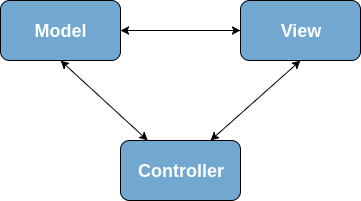
\includegraphics[width=0.7\textwidth]{imagenes/img_mvc}
	\caption{Diagrama Model-View-Controller.}
	\label{fig:img_mvc}
\end{figure}

\subsection{Django}
La decisión de usar el framework \textbf{Django} viene dada por su uso de la arquitectura MVC y su disponibilidad para trabajar con Python. Debido a que el controlador es manejado por el mismo framework y la parte más importante se produce en los modelos, las plantillas y las vistas, Django es conocido como un Framework MTV (Model- View - Template) \cite{cita_mvt}.
\begin{itemize}
	\item \textbf{Modelo} (Model): \textbf{información} con la que trabaja el sistema. Se encarga de gestionar los accesos a dicha información, tanto consultas como actualizaciones. Se corresponde con la base de datos.
	\item \textbf{Vista} (View): esta capa contiene la \textbf{lógica} que accede al modelo y la delega a la plantilla apropiada: actúa como puente entre el modelos y las plantillas.
	\item \textbf{Plantilla} (Template): se relaciona con la \textbf{presentación} de la información: como algunas cosas son mostradas sobre una página web u otro tipo de documento. \\
\end{itemize}

\begin{figure}[H]
	\centering
	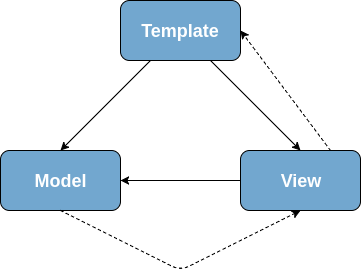
\includegraphics[width=0.7\textwidth]{imagenes/img_mvt}
	\caption{Diagrama Model-View-Template.}
	\label{fig:img_mvt}
\end{figure}

Django nos permite crear sitios web complejos ofreciendo diversos componentes que podemos usar para el desarrollo de nuestra aplicación.

\subsection{Sistema gestor de base de datos}
El sistema gestor de base de datos es el encargado de proporcionar la capa de acceso a la información de la base de datos. Haciendo uso del ORM de Django, utilizaremos un conector para la base de datos \textbf{MongoDB}.

\section{Frontend}
El \textbf{frontend} se refiere a la parte del sistema que se encarga de interactuar con los usuarios y mandar las peticiones al backend. Para interactuar con los usuarios hacemos uso de tecnologías web como \textbf{HTML}, \textbf{CSS} y \textbf{Javascript}. Este sistema trabaja todo el tiempo recibiendo peticiones de usuarios, por lo tanto usando las tecnologías mencionadas y añadiendo otras, como \textbf{jQuery}, haremos de nuestra interfaz un entorno intuitivo para los usuarios. \\

\subsection{jQuery}
\textbf{jQuery} es una librería de Javascript la cual ofrece la posibilidad de manipular los documentos HTML y manejar eventos, dotando a la web de una mayor dinamicidad. Es compatible con la mayoría de los navegadores actuales, tanto en pc como en dispositivos móviles. \\

\subsection{AJAX}
Por otro lado \textbf{AJAX} nos brinda la oportunidad de cargar datos desde el backend sin la necesidad de recargar toda la página del navegador. \\

\subsection{Twitter Bootstrap}
Otra tecnología usada de cara a la interacción con los usuarios de nuestra aplicación es la que nos aporta \textbf{Twitter Bootstrap}. Twitter Bootstrap es un framework CSS que nos facilita la tarea del diseño de la aplicación. Con esta tecnología podremos crear diseños muy elegantes y limpios, además de dotar a la aplicación web de un diseño adaptativo (responsive design) y así poder disfrutar de nuestra aplicación sin problemas en cualquier dispositivo y tamaño de pantalla. \\
